\input ../talk-header.tex
\title{Machine Learning}
\subtitle{Introduction, Data, Modeling}

% If you wish to uncover everything in a step-wise fashion, uncomment
% the following command: 
%\beamerdefaultoverlayspecification{<+->}

\begin{document}

\begin{frame}
  \titlepage
\end{frame}

\begin{frame}
  % https://static.pexels.com/photos/105855/pexels-photo-105855.jpeg
  % CC0 license.
  \cimgw{child-blocks.jpg}
\end{frame}

\begin{frame}
  % https://static.pexels.com/photos/194087/pexels-photo-194087.jpeg
  % https://www.pexels.com/photo/man-wearing-silver-skull-ring-194087/
  % CC0 license.
  \cimgw{man-wearing-silver-skull-ring.jpg}
\end{frame}

\begin{frame}
  % https://static.pexels.com/photos/249/black-and-white-trees-winter-branches.jpg
  % CC0 license.
  \vspace{-3.5cm}\cimgw{black-and-white-trees-winter-branches.jpg}
\end{frame}

\begin{frame}
  \vphrase{Supervised}
\end{frame}

\begin{frame}
  \vphrase{Unsupervised}
\end{frame}

\begin{frame}
  \vphrase{Reinforcement}
\end{frame}

\begin{frame}
  % https://www.pexels.com/photo/person-high-five-india-14796/
  % https://static.pexels.com/photos/14796/pexels-photo.jpg
  % CC0 license
  \cimgw{high-five-india.jpg}
\end{frame}

\begin{frame}
  \frametitle{Course structure}
  \only<1>{
    Ten afternoons:
    \begin{itemize}
    \item     8, 22 Nov
    \item     6, Dec
    \item     10, 24 Jan
    \item     14, 28 Feb
    \item     14, 28 Mar
    \item     11 Apr
    \end{itemize}
  }
  \only<2>{
    \begin{itemize}
    \item Email \url{jeff@p27.eu}
    \item Mailing list: \url{ml-week-2017-11@googlegroups.com}
    \item Github: \url{https://github.com/mlweek/MLWeek_v3}
    \end{itemize}
  }
\end{frame}

\begin{frame}
  \vphrase{Curse of Dimensionality}
\end{frame}

\begin{frame}
  \only<1>{
    \vphrase{Machine learning is not magic}
  }
  \only<2>{
    \vphrase{Machine learning is mathematics}
  }
  \only<3>{
    \vspace{1cm}
    \blue{\bf Mostly, it's these maths:}
    \begin{itemize}
    \item Probability
    \item Statistics
    \item Linear algebra
    \item Optimisation theory
    \item Differential calculus
    \end{itemize}
    \bigskip
    \purple{Unless you want to, we'll skip the maths.}
  }
\end{frame}

\talksection{Probability}

\begin{frame}
  \frametitle{Probability}
  \phrase{events}
  \begin{itemize}
  \item independent
  \item dependent
  \end{itemize}
\end{frame}

\talksection{Statistics}

\begin{frame}[t]
  \frametitle{What is Statistics}
  
  \begin{enumerate}
  \item<1-3> Identify a question or problem.
  \item<1-3> Collect relevant data on the topic.
  \item<1-3> Analyze the data.
  \item<1-3> Form a conclusion.
  \end{enumerate}
  \only<2>{Sadly, sometimes people forget 1.}
  \only<3>{Statistics is about making 2--4 efficient, rigorous, and meaningful.}
  \only<3>{\vfill\prevwork{\textit{OpenIntro Statistics},
      2nd edition, D.~Diez, C.~Barr, M.~Çetinkaya-Rundel, 2013.}}
\end{frame}

\begin{frame}[t]
  \frametitle{What is data science?}

  \only<1-4>{(Exercise: Is this the same question as the last slide?)}

  \only<1>{
    \begin{enumerate}
    \item Define the question of interest
    \item Get the data
    \item Clean the data
    \item Explore the data
    \item Fit statistical models
    \item Communicate the results
    \item Make your analysis reproducible
    \end{enumerate}
  }
  \only<2>{
    \begin{enumerate}
    \item Define the question of interest
    \item Get the data
    \item Clean the data
    \item \purple{Explore the data}
    \item \purple{Fit statistical models}
    \item Communicate the results
    \item Make your analysis reproducible
    \end{enumerate}

    \blue{What the public thinks.}
  }
  \only<3>{
    \begin{enumerate}
    \item Define the question of interest
    \item \purple{Get the data}
    \item \purple{Clean the data}
    \item Explore the data
    \item Fit statistical models
    \item \purple{Communicate the results}
    \item \purple{Make your analysis reproducible}
    \end{enumerate}

    \blue{Where we spend most of our time.}
  }
  \only<4>{
    \begin{enumerate}
    \item \purple{Define the question of interest}
    \item Get the data
    \item Clean the data
    \item Explore the data
    \item Fit statistical models
    \item Communicate the results
    \item Make your analysis reproducible
    \end{enumerate}

    \blue{The easiest part to forget.}
  }
  \only<5>{\vfill\prevwork{\url{http://simplystatistics.org/2015/03/17/} \url{data-science-done-well-looks-easy-and-that-is-a-big-} \url{problem-for-data-scientists/}}}

  \only<6>{\vfill\cimgg{model-in-one-day.jpg}\vfill}
\end{frame}

\begin{frame}
  \frametitle{Anecdote}

  Some properties of anecdote:
  
  \begin{itemize}
  \item is data
  \item haphazardly collected
  \item is generally not representative
  \item sometimes result of selective retention
  \item does not accumulate to be representative
  \item might be true (by chance)
  \item is ok to use as hypothesis, but be clear that hypothesis is anecdote
  \end{itemize}
\end{frame}

\begin{frame}
  \frametitle{Study Types}

  \begin{itemize}
  \item Observational
  \item Experimental
  \end{itemize}
  
  \only<2>{
    What can go wrong?
    \begin{itemize}
    \item Forgetting that association $\ne$ causation
    \item Not random
    \item Confounding variables
    \end{itemize}
  }
\end{frame}

\begin{frame}
  \frametitle{Variable types}
  \cimg{variable-types.png}
\end{frame}

\begin{frame}
  \cimggg{bias-variance.png}
\end{frame}

\begin{frame}
  \frametitle{Mean}

  \begin{itemize}
  \item Weighted and unweighted
  \item Centroid to physicists
  \end{itemize}

  \only<2-4> {
    \cimgg{teeter-totter.png}
  }
  \only<3>{
    \begin{displaymath}
      \mu = E(X) = \sum w_i x_i = \mathbf{w\cdot x}
    \end{displaymath}

    \vfill
    \prevwork{\url{http://telescopes.stardate.org/images/research/teeter-totter/TT4.gif}}
  }
  \only<4>{
    \begin{displaymath}
      \mu = E(X) = \sum \Pr(X=x_i) x_i
    \end{displaymath}

    \vfill
    \prevwork{\url{http://telescopes.stardate.org/images/research/teeter-totter/TT4.gif}}
  }
  \only<5>{
    \begin{displaymath}
      \mu = E(X) = \int xf(x) \D{x}
    \end{displaymath}

    \vfill
    \prevwork{\url{http://telescopes.stardate.org/images/research/teeter-totter/TT4.gif}}
  }
  \only<6>{
    \cimgg{centroid-hanging-discrete.png}
  }
  \only<7>{
    \cimgg{centroid-balance-continuous.png}
  }
\end{frame}

\begin{frame}
  \frametitle{Population statistics}

  \soloo{1}{\textbf{Deviation} is distance from mean.}
  \soloo{2}{\textbf{Variance} is mean square of deviations}
  \soloo{3}{\textbf{Standard deviation} is square root of variance}

  \only<4>{
    \vfill
    \begin{displaymath}
      s^2 = \frac{(\overline x - x_1)^2 + \dotsb (\overline x - x_n)^2}{n-1}
    \end{displaymath}
  }
  \only<5>{
    \vfill
    \begin{displaymath}
      \sigma^2 = \frac{(\overline x - x_1)^2 + \dotsb (\overline x - x_n)^2}{n}
    \end{displaymath}
  }
  \only<6>{
    \vfill
    \begin{displaymath}
      \mbox{Var}(X) = \sigma^2 = (\overline x - x_1)^2 \Pr(X=x_1) + \dotsb
        (\overline x - x_n)^2 \Pr(X=x_n)
    \end{displaymath}
  }
\end{frame}

\begin{frame}
  \cimghh{boxplot-vs-pdf.png}
\end{frame}

\begin{frame}
  \frametitle{Evaluating Normal Approximations}

  \only<1>{Easy technique 1: visually compare to normal plot.

    \cimghhh{normal-plot.png}
  }

  \only<2> {Easy technique 2: normal probability plot.

    \cimghhhh{normal-quantile.png}

    \vspace{-7mm}
    Also known as a quantile-quantile plot.
  }
\end{frame}

\begin{frame}
  \vfill
  \begin{displaymath}
    \overline{x}\ne\mu
  \end{displaymath}
  \vfill
\end{frame}

\begin{frame}
  \frametitle{Inference Concepts}

  \only<1->{\textbf{Running mean.}  Sequence of partial sums (divided
    by number in sum).
  }

  \only<2>{
    \bigskip
    \cimgg{running-mean.png}
  }

  \only<3->{\textbf{Sampling variation.}  Change of $\overline x$ from
    one sample to the next.
  }

  \only<4->{\textbf{Sampling distribution.}  The distribution of
    possible point samples of a fixed size from a given population.
  }
\end{frame}

\begin{frame}
  \frametitle{Sampling distribution}

  \cimg{sampling-distribution.png}
\end{frame}

\begin{frame}
  \frametitle{Confidence intervals}

  Sample $n$ points, choose an interval around the sample mean.

  A 95\% confidence interval means if we sample repeatedly, about 95\%
  of the samples will contain the population mean.

  \only<2>{
    \cimghhhh{confidence-intervals.png}
  }

  \only<3>{
    \cimghhhh{confidence-intervals-2.png}
  }
\end{frame}


\talksection{Linear Algebra}

\begin{frame}
  \frametitle{Linear algebra: basics}
  \only<1>{
    \begin{displaymath}
      v = 
      \begin{pmatrix}
        v_1\\
        v_2\\
        \vdots\\
        v_n
      \end{pmatrix}
      \in \mathbb{R}^n
    \end{displaymath}
  }
  \only<2>{
    \begin{align*}
      A & = 
      \begin{bmatrix}
        a_{1,1} & a_{1,2} & a_{1,3} \\
        a_{2,1} & a_{2,2} & a_{2,3} \\
        a_{3,1} & a_{3,2} & a_{3,3}
      \end{bmatrix} 
      =
      \begin{pmatrix}
        a_{1,1} & a_{1,2} & a_{1,3} \\
        a_{2,1} & a_{2,2} & a_{2,3} \\
        a_{3,1} & a_{3,2} & a_{3,3}
      \end{pmatrix} \\[4mm]
      & =
      \begin{Bmatrix}
        a_{1,1} & a_{1,2} & a_{1,3} \\
        a_{2,1} & a_{2,2} & a_{2,3} \\
        a_{3,1} & a_{3,2} & a_{3,3}
      \end{Bmatrix}
      \in \mathbb{R}^{n\times n}
    \end{align*}
  }
  \only<3>{
    \begin{displaymath}
        u + v = 
      \begin{pmatrix}
        u_1 + v_1\\
        u_2 + v_2\\
        \vdots\\
        u_n + v_n
      \end{pmatrix}
    \end{displaymath}
  }
  \only<4>{
    \begin{displaymath}
      \alpha v =
      \begin{pmatrix}
        \alpha v_1\\
        \alpha  v_2\\
        \vdots\\
        \alpha v_n
      \end{pmatrix}
       \qquad (\alpha\in\mathbb{R})
    \end{displaymath}
  }
  \only<5>{
    \begin{displaymath}
      \parallel v\parallel = \sqrt{v_1^2 + \cdots + v_n^2}
    \end{displaymath}
  }
  \only<6>{
    \begin{align*}
      u\cdot v & = u_1\cdot v_1 + \dotsb + u_n \cdot v_n \\[4mm]
      & = \parallel u\parallel \parallel v\parallel \cos\theta
    \end{align*}
  }
  \only<7>{
    \begin{align*}
      C = A + B & \iff c_{ij} = a_{ij} + b_{ij} \\[5mm]
      %
      C = AB & \iff c_{ij} = \sum_k a_{ik}b_{kj} \\[5mm]
      %
      A = B^T & \iff a_{ij} = b_{ji}
    \end{align*}
    
    \begin{displaymath}
      AA^{-1} = A^{-1}A = \mathrm{diag}(1)      
    \end{displaymath}
  }
\end{frame}

\begin{frame}
  \frametitle{Linear algebra: transformations}
  \only<1>{
    \begin{align*}
      Ax = y & \hspace{1cm} f = T_A \,:\, \mathbb{R}^n\rightarrow \mathbb{R}^n \\[5mm]
      %
      x = A^{-1}Ax = A^{-1}y & \hspace{1cm} f^{-1} = T_{A^{-1}}
      \,:\, \mathbb{R}^n\rightarrow \mathbb{R}^n \\[5mm]
    \end{align*}
  }
  \only<2-3>{
    $B$ is a basis for $V$ iff any of these conditions are met:
    \begin{itemize}
    \item $B$ is a minimal generating set of $V$
    \item $B$ is a maximal set of linearly independent vectors
    \item Every vector $v\in V$ can be expressed in a unique way as a sum of $b_i\in B$
    \end{itemize}

    \purple{(The conditions are equivalent.)}

    \only<3>{\red{Bases are not unique.}}
  }
  \only<4-6>{Eigenvectors, eigenvalues:
    \begin{displaymath}
      Av = \lambda v
    \end{displaymath}

    \only<5>{
      \begin{displaymath}
        Av = \lambda 1 v \;\iff\; (A-\lambda 1)v = 0
      \end{displaymath}
    }
    \only<6>{
      Some matrices are diagonalisable.  Then
      \begin{align*}
        A = Q\Lambda Q^{-1} \hspace{1cm} \mbox{ with } \Lambda & =
        \begin{bmatrix}
          \lambda_1 & \cdots & 0 \\
          \vdots & \ddots & 0 \\
          0 & 0 & \lambda_n
        \end{bmatrix} \\[5mm]
        %
        \mbox{and } Q & =
        \begin{bmatrix}
          \mid && \mid \\
          v_1 & \cdots & v_n \\
          \mid && \mid
        \end{bmatrix}
      \end{align*}
    }
  }
  \only<7>{\vphrase{video time}}
\end{frame}

%%%%%%%%%%%%%%%%%%%%%%%%%%%%%%%%%%%%%%%%%%%%%%%%%%%%%%%%%%%%%%%%%%%%%%
%\talksection{Break}

\begin{frame}
  % https://static.pexels.com/photos/60117/match-sticks-lighter-sulfur-60117.jpeg
  % https://www.pexels.com/photo/matchess-60117/
  % CC0 license
  \cimgwb{match-sticks-lighter-sulfur.jpg}
  \vspace{-.8\textheight}
  \phrase{Questions?}

\end{frame}

\begin{frame}
  \vphrase{Features and Modeling}
\end{frame}

\begin{frame}
  \phrase{Vector spaces}

  \vspace{1cm}
  \only<2>{\centerline{Features are dimensions}}
\end{frame}

\begin{frame}
  \phrase{Feature extraction}

  \vspace{1cm}
  \phrase{Feature engineering}

  \only<2>{\vspace{3mm}\centerline{Synthetic features}}
\end{frame}

\begin{frame}
  \frametitle{Feature Engineering}
  \only<1>{
    \begin{enumerate}
    \item Brainstorm
    \item Pick some
    \item Make them
    \item Evaluate
    \item Repeat
    \end{enumerate}
  }
\end{frame}

\begin{frame}
  \vspace{4mm}
  
  \cimgh{titanic-titles.png}
  \vspace{-3mm}
  \prevwork{Kaggle}
\end{frame}

\begin{frame}
  \cimg{reading-time-1.png}
  \prevwork{Jellybooks}
\end{frame}

\begin{frame}
  \cimg{reading-time-2.png}
  \prevwork{Jellybooks}
\end{frame}

\begin{frame}
  \vphrase{One of $K$ = one-hot encoding}
\end{frame}

\begin{frame}
  \frametitle{Text features}
  \blue{Bag of words}
  \only<1>{
    \begin{itemize}
    \item Corpus (documents)
    \item Vocabulary (set of unique words)
    \item Words
    \end{itemize}
  }
  \only<2>{
    \begin{itemize}
    \item Order doesn't matter
    \item Stop words
    \item Stemming {\it(racinisation, désuffixation)}
    \item Lemmatisation {\it(transformer en lemme)}
    \end{itemize}
  }
\end{frame}

\begin{frame}
  \frametitle{Image features}
  \only<1>{
    \begin{itemize}
    \item Corners, edges (rotation invariant, but scaling can hide)
    \item More complex: scale space or RNN
    \item Point matching is easy
    \end{itemize}
  }
  \only<2>{
    Problems
    \begin{itemize}
    \item Illumination
    \item Scale
    \item Rotation
    \item Skew (perspective)
    \item Data size (matrices not sparse)
    \end{itemize}
  }
\end{frame}

\begin{frame}
  \frametitle{python}
  \only<1>{Useful tools
    \begin{itemize}
    \item virtualenv
    \item pip
    \item ipython
    \item ipython notebook
    \item \url{conda.pydata.org}
    \end{itemize}
  }
  \only<2>{Notes
    \begin{itemize}
    \item \texttt{pip install -r requirements.txt}
    \item ipython offers tab completion (vs python)
    \item ipython notebook opens in a browser, caches cell output but not cell state
    \end{itemize}
  }
\end{frame}

\begin{frame}
  \frametitle{pandas}
  \only<1>{\lstinputlisting{pandas_1.py}}
  \only<2>{\purple{\texttt{Dataframe} has many constructors.  For example,}
    \lstinputlisting{pandas_2.py}
  }
  \only<3>{\purple{Viewing data}
    \lstinputlisting{pandas_3.py}
  }
  \only<4>{\purple{Basic data exploration}
    \lstinputlisting{pandas_4.py}
  }
  \only<5>{\purple{Select a column (series)}
    \lstinputlisting{pandas_5.py}
  }
  \only<6>{\purple{Select a range}
    \lstinputlisting{pandas_6.py}
  }
  \only<7>{\purple{Boolean selection criteria}
    \lstinputlisting{pandas_7.py}
  }
  \only<8>{\purple{Recommended}
    
    \vspace{5mm}
    \url{http://www.gregreda.com/2013/10/26/intro-to-pandas-data-structures/}
  }
\end{frame}

\begin{frame}
  \frametitle{Plotting}
  \only<1>{\purple{Draw a line}
    \lstinputlisting{pyplot_1.py}
    \vspace{-19mm}
    \flushright{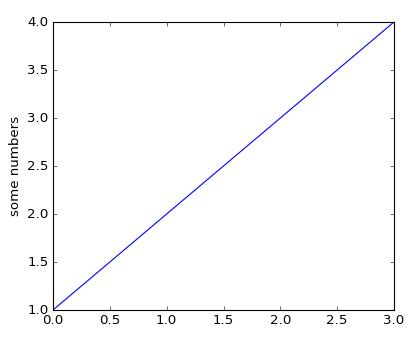
\includegraphics[width=.5\textwidth]{pyplot_1.png}}
  }
  \only<2>{\purple{Draw a line}
    \lstinputlisting{pyplot_2.py}
    \vspace{-19mm}
    \flushright{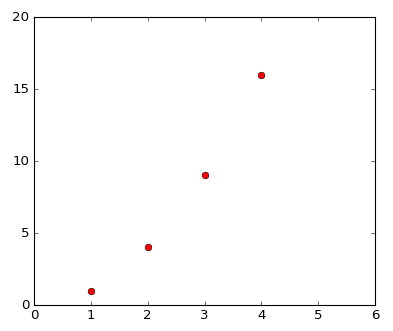
\includegraphics[width=.5\textwidth]{pyplot_2.png}}
  }
  \only<3>{\purple{Draw a line}
    \lstinputlisting{pyplot_3.py}
    \vspace{-55mm}
    \flushright{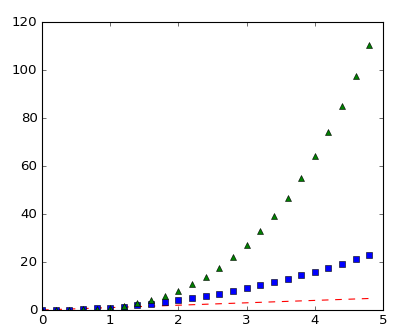
\includegraphics[width=.5\textwidth]{pyplot_3.png}}
  }
  \only<4>{\purple{Draw two curves}
    \lstinputlisting{pyplot_4.py}
  }
  \only<5>{
    \flushright{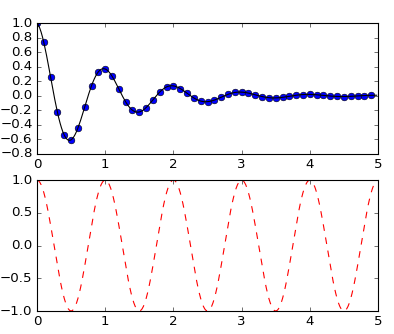
\includegraphics[width=.5\textwidth]{pyplot_4.png}}
  }    
  \only<6>{\purple{Draw two curves}
    \lstinputlisting{pyplot_5.py}
  }
  \only<7>{
    \flushright{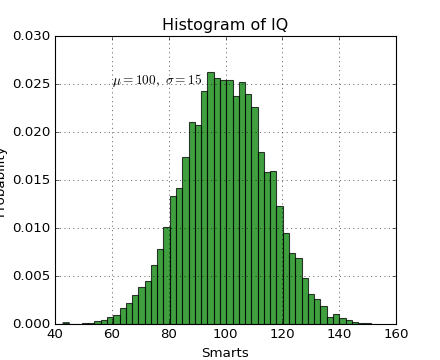
\includegraphics[width=.5\textwidth]{pyplot_5.png}}
  }
  \only<8>{\purple{Scatter plot}
    \prevwork{\url{http://matplotlib.org/mpl_examples/pylab_examples/scatter_demo2.py}}
    \lstinputlisting{pyplot_6.py}
    \vspace{-60mm}
    \flushright{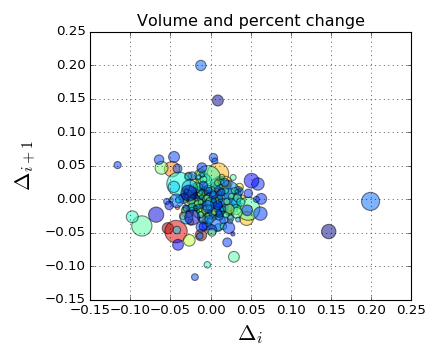
\includegraphics[width=.5\textwidth]{pyplot_6.png}}
    
  }
  \only<9>{
    \prevwork{\url{http://matplotlib.org/users/pyplot_tutorial.html}}
      
    \prevwork{\url{http://matplotlib.org/users/beginner.html}}
  }
\end{frame}

%%%%%%%%%%%%%%%%%%%%%%%%%%%%%%%%%%%%%%%%%%%%%%%%%%%%%%%%%%%%%%%%%%%%%%
%\talksection{Break}

\begin{frame}
  % https://www.pexels.com/photo/food-healthy-people-woman-41219/
  % https://static.pexels.com/photos/41219/apple-diet-face-food-41219.jpeg
  % CC0 license
  \cimgh{apple-pear.jpg}
  \vspace{-.6\textheight}
  \phrase{Questions?}
\end{frame}


\end{document}
